\PassOptionsToPackage{unicode=true}{hyperref} % options for packages loaded elsewhere
\PassOptionsToPackage{hyphens}{url}
%
\documentclass[]{article}
\usepackage{lmodern}
\usepackage{amssymb,amsmath}
\usepackage{ifxetex,ifluatex}
\usepackage{fixltx2e} % provides \textsubscript
\ifnum 0\ifxetex 1\fi\ifluatex 1\fi=0 % if pdftex
  \usepackage[T1]{fontenc}
  \usepackage[utf8]{inputenc}
  \usepackage{textcomp} % provides euro and other symbols
\else % if luatex or xelatex
  \usepackage{unicode-math}
  \defaultfontfeatures{Ligatures=TeX,Scale=MatchLowercase}
\fi
% use upquote if available, for straight quotes in verbatim environments
\IfFileExists{upquote.sty}{\usepackage{upquote}}{}
% use microtype if available
\IfFileExists{microtype.sty}{%
\usepackage[]{microtype}
\UseMicrotypeSet[protrusion]{basicmath} % disable protrusion for tt fonts
}{}
\IfFileExists{parskip.sty}{%
\usepackage{parskip}
}{% else
\setlength{\parindent}{0pt}
\setlength{\parskip}{6pt plus 2pt minus 1pt}
}
\usepackage{hyperref}
\hypersetup{
            pdftitle={Tests and ideas with new package},
            pdfauthor={Derek Corcoran},
            pdfborder={0 0 0},
            breaklinks=true}
\urlstyle{same}  % don't use monospace font for urls
\usepackage[margin=1in]{geometry}
\usepackage{color}
\usepackage{fancyvrb}
\newcommand{\VerbBar}{|}
\newcommand{\VERB}{\Verb[commandchars=\\\{\}]}
\DefineVerbatimEnvironment{Highlighting}{Verbatim}{commandchars=\\\{\}}
% Add ',fontsize=\small' for more characters per line
\usepackage{framed}
\definecolor{shadecolor}{RGB}{248,248,248}
\newenvironment{Shaded}{\begin{snugshade}}{\end{snugshade}}
\newcommand{\AlertTok}[1]{\textcolor[rgb]{0.94,0.16,0.16}{#1}}
\newcommand{\AnnotationTok}[1]{\textcolor[rgb]{0.56,0.35,0.01}{\textbf{\textit{#1}}}}
\newcommand{\AttributeTok}[1]{\textcolor[rgb]{0.77,0.63,0.00}{#1}}
\newcommand{\BaseNTok}[1]{\textcolor[rgb]{0.00,0.00,0.81}{#1}}
\newcommand{\BuiltInTok}[1]{#1}
\newcommand{\CharTok}[1]{\textcolor[rgb]{0.31,0.60,0.02}{#1}}
\newcommand{\CommentTok}[1]{\textcolor[rgb]{0.56,0.35,0.01}{\textit{#1}}}
\newcommand{\CommentVarTok}[1]{\textcolor[rgb]{0.56,0.35,0.01}{\textbf{\textit{#1}}}}
\newcommand{\ConstantTok}[1]{\textcolor[rgb]{0.00,0.00,0.00}{#1}}
\newcommand{\ControlFlowTok}[1]{\textcolor[rgb]{0.13,0.29,0.53}{\textbf{#1}}}
\newcommand{\DataTypeTok}[1]{\textcolor[rgb]{0.13,0.29,0.53}{#1}}
\newcommand{\DecValTok}[1]{\textcolor[rgb]{0.00,0.00,0.81}{#1}}
\newcommand{\DocumentationTok}[1]{\textcolor[rgb]{0.56,0.35,0.01}{\textbf{\textit{#1}}}}
\newcommand{\ErrorTok}[1]{\textcolor[rgb]{0.64,0.00,0.00}{\textbf{#1}}}
\newcommand{\ExtensionTok}[1]{#1}
\newcommand{\FloatTok}[1]{\textcolor[rgb]{0.00,0.00,0.81}{#1}}
\newcommand{\FunctionTok}[1]{\textcolor[rgb]{0.00,0.00,0.00}{#1}}
\newcommand{\ImportTok}[1]{#1}
\newcommand{\InformationTok}[1]{\textcolor[rgb]{0.56,0.35,0.01}{\textbf{\textit{#1}}}}
\newcommand{\KeywordTok}[1]{\textcolor[rgb]{0.13,0.29,0.53}{\textbf{#1}}}
\newcommand{\NormalTok}[1]{#1}
\newcommand{\OperatorTok}[1]{\textcolor[rgb]{0.81,0.36,0.00}{\textbf{#1}}}
\newcommand{\OtherTok}[1]{\textcolor[rgb]{0.56,0.35,0.01}{#1}}
\newcommand{\PreprocessorTok}[1]{\textcolor[rgb]{0.56,0.35,0.01}{\textit{#1}}}
\newcommand{\RegionMarkerTok}[1]{#1}
\newcommand{\SpecialCharTok}[1]{\textcolor[rgb]{0.00,0.00,0.00}{#1}}
\newcommand{\SpecialStringTok}[1]{\textcolor[rgb]{0.31,0.60,0.02}{#1}}
\newcommand{\StringTok}[1]{\textcolor[rgb]{0.31,0.60,0.02}{#1}}
\newcommand{\VariableTok}[1]{\textcolor[rgb]{0.00,0.00,0.00}{#1}}
\newcommand{\VerbatimStringTok}[1]{\textcolor[rgb]{0.31,0.60,0.02}{#1}}
\newcommand{\WarningTok}[1]{\textcolor[rgb]{0.56,0.35,0.01}{\textbf{\textit{#1}}}}
\usepackage{longtable,booktabs}
% Fix footnotes in tables (requires footnote package)
\IfFileExists{footnote.sty}{\usepackage{footnote}\makesavenoteenv{longtable}}{}
\usepackage{graphicx,grffile}
\makeatletter
\def\maxwidth{\ifdim\Gin@nat@width>\linewidth\linewidth\else\Gin@nat@width\fi}
\def\maxheight{\ifdim\Gin@nat@height>\textheight\textheight\else\Gin@nat@height\fi}
\makeatother
% Scale images if necessary, so that they will not overflow the page
% margins by default, and it is still possible to overwrite the defaults
% using explicit options in \includegraphics[width, height, ...]{}
\setkeys{Gin}{width=\maxwidth,height=\maxheight,keepaspectratio}
\setlength{\emergencystretch}{3em}  % prevent overfull lines
\providecommand{\tightlist}{%
  \setlength{\itemsep}{0pt}\setlength{\parskip}{0pt}}
\setcounter{secnumdepth}{5}
% Redefines (sub)paragraphs to behave more like sections
\ifx\paragraph\undefined\else
\let\oldparagraph\paragraph
\renewcommand{\paragraph}[1]{\oldparagraph{#1}\mbox{}}
\fi
\ifx\subparagraph\undefined\else
\let\oldsubparagraph\subparagraph
\renewcommand{\subparagraph}[1]{\oldsubparagraph{#1}\mbox{}}
\fi

% set default figure placement to htbp
\makeatletter
\def\fps@figure{htbp}
\makeatother

\usepackage{booktabs}
\usepackage{longtable}
\usepackage{array}
\usepackage{multirow}
\usepackage{wrapfig}
\usepackage{float}
\usepackage{colortbl}
\usepackage{pdflscape}
\usepackage{tabu}
\usepackage{threeparttable}
\usepackage{threeparttablex}
\usepackage[normalem]{ulem}
\usepackage{makecell}
\usepackage{xcolor}

\title{Tests and ideas with new package}
\author{Derek Corcoran}
\date{2020-02-26}

\begin{document}
\maketitle

\hypertarget{load-packages}{%
\section{Load packages}\label{load-packages}}

I will load a bunch of packages including \emph{ggraph} to ilustrate the network, in particular the Phillips Problem.

\begin{Shaded}
\begin{Highlighting}[]
\KeywordTok{library}\NormalTok{(dispRsal)}
\KeywordTok{library}\NormalTok{(kableExtra)}
\KeywordTok{library}\NormalTok{(gdistance)}
\KeywordTok{library}\NormalTok{(ggraph)}
\KeywordTok{library}\NormalTok{(igraph)}
\KeywordTok{library}\NormalTok{(lpSolve)}
\KeywordTok{library}\NormalTok{(magrittr)}
\KeywordTok{library}\NormalTok{(raster)}
\KeywordTok{library}\NormalTok{(tidyverse)}
\end{Highlighting}
\end{Shaded}

\hypertarget{the-phillips-problem}{%
\section{The Phillips problem}\label{the-phillips-problem}}

This problem starts with a toy model of a species. We have modeled the distribution of that species and we have projected that distribution through 2 different time-slices T0 and T1, this is conceptualized by the following rasterstack called \emph{Phillips}, as seen in Figure \ref{fig:PhilDist}

\begin{Shaded}
\begin{Highlighting}[]
\KeywordTok{plot}\NormalTok{(Phillips)}
\end{Highlighting}
\end{Shaded}

\begin{figure}
\centering
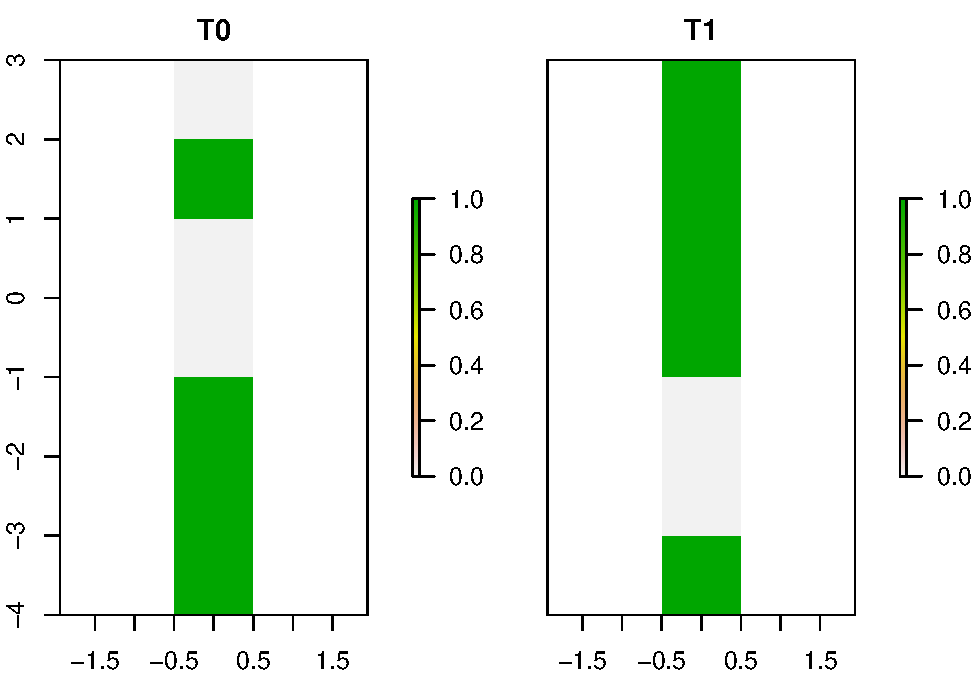
\includegraphics{Ideas2_files/figure-latex/PhilDist-1.pdf}
\caption{\label{fig:PhilDist}Predicted distribution of a species for two time slices, green means the species is predicted to be present, and grey that the species is predicted to be absent}
\end{figure}

Fot that same area we have a costlayer (\emph{PhilCost}), we but the two middle cells are unavailable for the species, because there is an obstacle there (eg: a city or a glaciar) as seen in Figure \ref{fig:Cost}

\begin{figure}
\centering
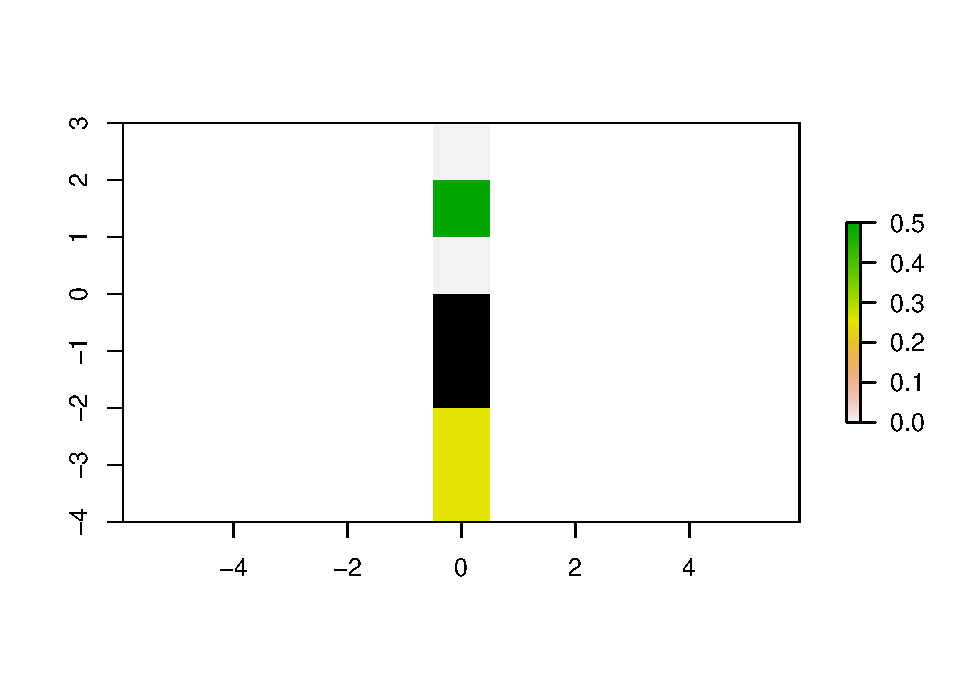
\includegraphics{Ideas2_files/figure-latex/Cost-1.pdf}
\caption{\label{fig:Cost}Raster with the cost of buying each cell, black cells are unavailable cells}
\end{figure}

The idea is to create a solution where the species has always at least two cells (\emph{nchains}) available at each time-slice, but those cells have to be within reach for the species between time-slices. Let's say for example that for this species, the distance the species can travel is 111 km between time-slice 0 to time-slice 1, in this case the species would only be able to move to one adyacent cell between time-slices, this will be defined by the following variables:

\begin{Shaded}
\begin{Highlighting}[]
\NormalTok{layers_habitat =}\StringTok{ }\NormalTok{Phillips}
\NormalTok{layer_cost =}\StringTok{ }\NormalTok{PhilCost}
\NormalTok{Dist =}\StringTok{ }\DecValTok{111000}
\NormalTok{nchains =}\StringTok{ }\DecValTok{2}
\end{Highlighting}
\end{Shaded}

\hypertarget{step-1}{%
\section{Step 1}\label{step-1}}

First we eliminate the NA sites created by the unavailable areas shown in figure \ref{fig:Cost}

\begin{Shaded}
\begin{Highlighting}[]
\NormalTok{layers_habitat <-}\StringTok{ }\NormalTok{layers_habitat }\OperatorTok{*}\StringTok{ }\OperatorTok{!}\KeywordTok{is.na}\NormalTok{(layer_cost)}
\end{Highlighting}
\end{Shaded}

This will modify the raster shown in figure 1 \ref{fig:PhilDist} into the one we see in figure \ref{fig:ModHab}, notice that we lost 2 cells that use to be available when we first looked at the data.

\begin{Shaded}
\begin{Highlighting}[]
\NormalTok{layers_habitat <-}\StringTok{ }\NormalTok{layers_habitat }\OperatorTok{*}\StringTok{ }\OperatorTok{!}\KeywordTok{is.na}\NormalTok{(layer_cost)}
\end{Highlighting}
\end{Shaded}

\begin{figure}
\centering
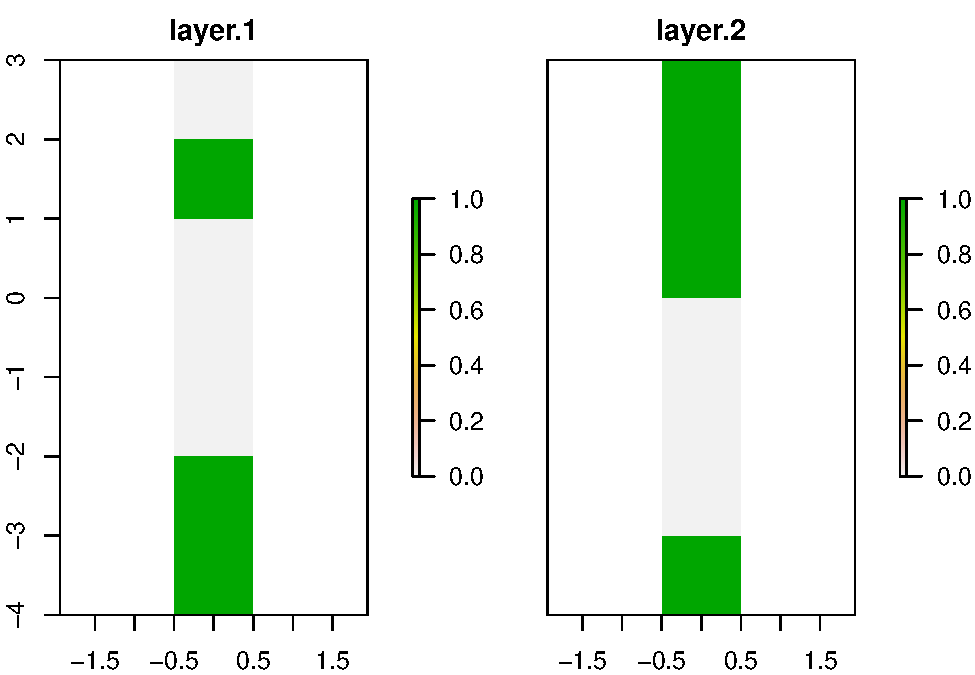
\includegraphics{Ideas2_files/figure-latex/ModHab-1.pdf}
\caption{\label{fig:ModHab}Habitat layers modified so that we take out the non available values}
\end{figure}

Then we create a data frame of all the nodes, as we see in table \ref{tab:A}, a new \emph{Cell\_id} was generated that is unique to every node in each time-slice, but the raster\_id was kept in order to be able to get the results back to the raster.

\begin{Shaded}
\begin{Highlighting}[]
\NormalTok{df_habitat <-}\StringTok{ }\KeywordTok{map_dfr}\NormalTok{(}\DataTypeTok{layers_habitat =}\NormalTok{ layers_habitat, }\DataTypeTok{.x =} \DecValTok{1}\OperatorTok{:}\KeywordTok{nlayers}\NormalTok{(layers_habitat), }
    \DataTypeTok{.f =} \OperatorTok{~}\NormalTok{layers_habitat[[.x]] }\OperatorTok\StringTok{ }\KeywordTok{values}\NormalTok{() }\OperatorTok\StringTok{ }\KeywordTok{tibble}\NormalTok{(}\DataTypeTok{habitat =}\NormalTok{ .) }\OperatorTok\StringTok{ }\KeywordTok{transmute}\NormalTok{(}\DataTypeTok{cell_id =} \KeywordTok{row_number}\NormalTok{(), }
        \DataTypeTok{time =}\NormalTok{ .x, }\DataTypeTok{habitat =}\NormalTok{ habitat)) }\OperatorTok\StringTok{ }\CommentTok{# give the same cell in different time slices different IDs}
\KeywordTok{mutate}\NormalTok{(}\DataTypeTok{raster_id =}\NormalTok{ cell_id, }\DataTypeTok{cell_id =}\NormalTok{ cell_id }\OperatorTok{+}\StringTok{ }\KeywordTok{max}\NormalTok{(cell_id) }\OperatorTok{*}\StringTok{ }\NormalTok{time)}
\end{Highlighting}
\end{Shaded}

\begin{table}[!h]

\caption{\label{tab:A}Nodes with a new cell id that is unique for every time slice, the raster id is also kept so that we can get the results back to the raster}
\centering
\begin{tabular}[t]{rrrr}
\toprule
cell\_id & time & habitat & raster\_id\\
\midrule
\rowcolor{gray!6}  8 & 1 & 0 & 1\\
9 & 1 & 1 & 2\\
\rowcolor{gray!6}  10 & 1 & 0 & 3\\
11 & 1 & 0 & 4\\
\rowcolor{gray!6}  12 & 1 & 0 & 5\\
\addlinespace
13 & 1 & 1 & 6\\
\rowcolor{gray!6}  14 & 1 & 1 & 7\\
15 & 2 & 1 & 1\\
\rowcolor{gray!6}  16 & 2 & 1 & 2\\
17 & 2 & 1 & 3\\
\addlinespace
\rowcolor{gray!6}  18 & 2 & 0 & 4\\
19 & 2 & 0 & 5\\
\rowcolor{gray!6}  20 & 2 & 0 & 6\\
21 & 2 & 1 & 7\\
\bottomrule
\end{tabular}
\end{table}

\hypertarget{generate-a-df-that-keeps-the-id-of-the-raster-cell-and-the-new-cell-id}{%
\section{Generate a DF that keeps the ID of the raster cell and the new cell ID}\label{generate-a-df-that-keeps-the-id-of-the-raster-cell-and-the-new-cell-id}}

In order to be able to compare the cell\_id with raster\_id in further tables a table was created with this use in mind, this is seen in table \ref{tab:IDs}:

\begin{Shaded}
\begin{Highlighting}[]
\NormalTok{df_IDs <-}\StringTok{ }\NormalTok{df_habitat }\OperatorTok\StringTok{ }\KeywordTok{rename}\NormalTok{(}\DataTypeTok{node_to =}\NormalTok{ cell_id) }\OperatorTok\StringTok{ }\NormalTok{dplyr}\OperatorTok{::}\KeywordTok{select}\NormalTok{(node_to, raster_id)}
\end{Highlighting}
\end{Shaded}

\begin{table}[!h]

\caption{\label{tab:IDs}Table of cell ID and Raster ID equivalencies}
\centering
\begin{tabular}[t]{rr}
\toprule
node\_to & raster\_id\\
\midrule
\rowcolor{gray!6}  8 & 1\\
9 & 2\\
\rowcolor{gray!6}  10 & 3\\
11 & 4\\
\rowcolor{gray!6}  12 & 5\\
\addlinespace
13 & 6\\
\rowcolor{gray!6}  14 & 7\\
15 & 1\\
\rowcolor{gray!6}  16 & 2\\
17 & 3\\
\addlinespace
\rowcolor{gray!6}  18 & 4\\
19 & 5\\
\rowcolor{gray!6}  20 & 6\\
21 & 7\\
\bottomrule
\end{tabular}
\end{table}

\hypertarget{generate-a-df-with-the-costs-of-each-cell}{%
\subsubsection{Generate a DF with the costs of each cell}\label{generate-a-df-with-the-costs-of-each-cell}}

Using the cost layer seen in figure \ref{fig:Cost} we generate a table with the cost of each node as seen in table table \ref{tab:CostTable}, this could be made smaller by only using the values of each cell and then using \ref{tab:IDs} to reference the cost

\begin{Shaded}
\begin{Highlighting}[]
\NormalTok{df_cost <-}\StringTok{ }\NormalTok{layer_cost }\OperatorTok\StringTok{ }\KeywordTok{values}\NormalTok{() }\OperatorTok\StringTok{ }\KeywordTok{tibble}\NormalTok{(}\DataTypeTok{cost =}\NormalTok{ .) }\OperatorTok\StringTok{ }\KeywordTok{mutate}\NormalTok{(}\DataTypeTok{cell_id =} \KeywordTok{row_number}\NormalTok{())}
\NormalTok{df_cost <-}\StringTok{ }\KeywordTok{map_dfr}\NormalTok{(}\DataTypeTok{df_cost =}\NormalTok{ df_cost, }\DataTypeTok{.x =} \DecValTok{1}\OperatorTok{:}\KeywordTok{nlayers}\NormalTok{(layers_habitat), }\DataTypeTok{.f =} \OperatorTok{~}\NormalTok{df_cost }\OperatorTok\StringTok{ }
\StringTok{    }\KeywordTok{transmute}\NormalTok{(}\DataTypeTok{cell_id =}\NormalTok{ cell_id }\OperatorTok{+}\StringTok{ }\KeywordTok{max}\NormalTok{(cell_id) }\OperatorTok{*}\StringTok{ }\NormalTok{.x, }\DataTypeTok{edge_cost =}\NormalTok{ cost))}
\end{Highlighting}
\end{Shaded}

\begin{table}[!h]

\caption{\label{tab:CostTable}Cost of every node}
\centering
\begin{tabular}[t]{rr}
\toprule
cell\_id & edge\_cost\\
\midrule
\rowcolor{gray!6}  8 & 0.00\\
9 & 0.50\\
\rowcolor{gray!6}  10 & 0.00\\
11 & NA\\
\rowcolor{gray!6}  12 & NA\\
\addlinespace
13 & 0.25\\
\rowcolor{gray!6}  14 & 0.25\\
15 & 0.00\\
\rowcolor{gray!6}  16 & 0.50\\
17 & 0.00\\
\addlinespace
\rowcolor{gray!6}  18 & NA\\
19 & NA\\
\rowcolor{gray!6}  20 & 0.25\\
21 & 0.25\\
\bottomrule
\end{tabular}
\end{table}

\hypertarget{getting-the-distances-between-variables}{%
\section{Getting the distances between variables}\label{getting-the-distances-between-variables}}

For that we use the function \texttt{edge\_distance\_limit} this will give use table \ref{tab:cons}, in which we have the pair of nodes and the distance between them in thre raster, this has already filtered out any distances greater than \texttt{Dist}

\begin{Shaded}
\begin{Highlighting}[]
\NormalTok{connections <-}\StringTok{ }\KeywordTok{edge_distance_limit}\NormalTok{(}\DataTypeTok{layer_cost =}\NormalTok{ PhilCost, }\DataTypeTok{layers_habitat =}\NormalTok{ Phillips, }
    \DataTypeTok{Dist =}\NormalTok{ Dist)}
\end{Highlighting}
\end{Shaded}

\begin{table}[!h]

\caption{\label{tab:cons}Edgelist of pairs of nodes among times including distance in meters}
\centering
\begin{tabular}[t]{rrr}
\toprule
dist & node\_from & node\_to\\
\midrule
\rowcolor{gray!6}  0.0 & 8 & 15\\
110575.7 & 8 & 16\\
\rowcolor{gray!6}  110575.7 & 9 & 15\\
0.0 & 9 & 16\\
\rowcolor{gray!6}  110574.6 & 9 & 17\\
\addlinespace
110574.6 & 10 & 16\\
\rowcolor{gray!6}  0.0 & 10 & 17\\
0.0 & 13 & 20\\
\rowcolor{gray!6}  110577.3 & 13 & 21\\
110577.3 & 14 & 20\\
\addlinespace
\rowcolor{gray!6}  0.0 & 14 & 21\\
0.0 & 15 & 22\\
\rowcolor{gray!6}  110575.7 & 15 & 23\\
110575.7 & 16 & 22\\
\rowcolor{gray!6}  0.0 & 16 & 23\\
\addlinespace
110574.6 & 16 & 24\\
\rowcolor{gray!6}  110574.6 & 17 & 23\\
0.0 & 17 & 24\\
\rowcolor{gray!6}  0.0 & 20 & 27\\
110577.3 & 20 & 28\\
\addlinespace
\rowcolor{gray!6}  110577.3 & 21 & 27\\
0.0 & 21 & 28\\
\bottomrule
\end{tabular}
\end{table}

\hypertarget{get-all-valid-edge-connections}{%
\section{get all valid edge connections,}\label{get-all-valid-edge-connections}}

In this step we do 3 different processes

First we filter only the pairs of nodes that hava a capacity of one:

\begin{Shaded}
\begin{Highlighting}[]
\NormalTok{edges_timesteps <-}\StringTok{ }\KeywordTok{map_dfr}\NormalTok{(}\DataTypeTok{df_habitat =}\NormalTok{ df_habitat, }\DataTypeTok{.x =} \DecValTok{2}\OperatorTok{:}\KeywordTok{nlayers}\NormalTok{(layers_habitat), }
    \DataTypeTok{.f =} \OperatorTok{~}\KeywordTok{expand_grid}\NormalTok{(}\DataTypeTok{node_from =}\NormalTok{ df_habitat }\OperatorTok\StringTok{ }\KeywordTok{filter}\NormalTok{(time }\OperatorTok{==}\StringTok{ }\NormalTok{.x }\OperatorTok{-}\StringTok{ }\DecValTok{1} \OperatorTok{&}\StringTok{ }\NormalTok{habitat }\OperatorTok{==}\StringTok{ }
\StringTok{        }\DecValTok{1}\NormalTok{) }\OperatorTok\StringTok{ }\KeywordTok{pull}\NormalTok{(cell_id), }\DataTypeTok{node_to =}\NormalTok{ df_habitat }\OperatorTok\StringTok{ }\KeywordTok{filter}\NormalTok{(time }\OperatorTok{==}\StringTok{ }\NormalTok{.x }\OperatorTok{&}\StringTok{ }\NormalTok{habitat }\OperatorTok{==}\StringTok{ }
\StringTok{        }\DecValTok{1}\NormalTok{) }\OperatorTok\StringTok{ }\KeywordTok{pull}\NormalTok{(cell_id), }\DataTypeTok{timeslice_to =}\NormalTok{ .x)) }\OperatorTok\StringTok{ }\KeywordTok{mutate}\NormalTok{(}\DataTypeTok{edge_id =} \KeywordTok{row_number}\NormalTok{(), }
    \DataTypeTok{edge_capacity =} \DecValTok{1}\NormalTok{, }\DataTypeTok{edge_cost =} \OtherTok{NA}\NormalTok{)}
\end{Highlighting}
\end{Shaded}

Then we add the cost by adding the costs of both nodes that participate in the edge:

\begin{Shaded}
\begin{Highlighting}[]
\ControlFlowTok{for}\NormalTok{ (i }\ControlFlowTok{in} \DecValTok{1}\OperatorTok{:}\KeywordTok{nrow}\NormalTok{(edges_timesteps)) \{}
    \CommentTok{# Check if the raster ID is equal in node_to and node_from}
    \ControlFlowTok{if}\NormalTok{ (df_IDs}\OperatorTok{$}\NormalTok{raster_id[df_IDs}\OperatorTok{$}\NormalTok{node_to }\OperatorTok{==}\StringTok{ }\NormalTok{edges_timesteps[i, ]}\OperatorTok{$}\NormalTok{node_to] }\OperatorTok{==}\StringTok{ }\NormalTok{df_IDs}\OperatorTok{$}\NormalTok{raster_id[df_IDs}\OperatorTok{$}\NormalTok{node_to }\OperatorTok{==}\StringTok{ }
\StringTok{        }\NormalTok{edges_timesteps[i, ]}\OperatorTok{$}\NormalTok{node_from]) \{}
        \CommentTok{## If that is the case just add the cost once}
\NormalTok{        edges_timesteps}\OperatorTok{$}\NormalTok{edge_cost[i] <-}\StringTok{ }\NormalTok{df_cost}\OperatorTok{$}\NormalTok{edge_cost[df_cost}\OperatorTok{$}\NormalTok{cell_id }\OperatorTok{==}\StringTok{ }\NormalTok{edges_timesteps[i, }
\NormalTok{            ]}\OperatorTok{$}\NormalTok{node_from]}
\NormalTok{    \}}
    \CommentTok{# Check if the raster ID is Different in node_to and node_from}
    \ControlFlowTok{if}\NormalTok{ (df_IDs}\OperatorTok{$}\NormalTok{raster_id[df_IDs}\OperatorTok{$}\NormalTok{node_to }\OperatorTok{==}\StringTok{ }\NormalTok{edges_timesteps[i, ]}\OperatorTok{$}\NormalTok{node_to] }\OperatorTok{!=}\StringTok{ }\NormalTok{df_IDs}\OperatorTok{$}\NormalTok{raster_id[df_IDs}\OperatorTok{$}\NormalTok{node_to }\OperatorTok{==}\StringTok{ }
\StringTok{        }\NormalTok{edges_timesteps[i, ]}\OperatorTok{$}\NormalTok{node_from]) \{}
        \CommentTok{## If that is the case just add the cost twice}
\NormalTok{        edges_timesteps}\OperatorTok{$}\NormalTok{edge_cost[i] <-}\StringTok{ }\NormalTok{df_cost}\OperatorTok{$}\NormalTok{edge_cost[df_cost}\OperatorTok{$}\NormalTok{cell_id }\OperatorTok{==}\StringTok{ }\NormalTok{edges_timesteps[i, }
\NormalTok{            ]}\OperatorTok{$}\NormalTok{node_from] }\OperatorTok{+}\StringTok{ }\NormalTok{df_cost}\OperatorTok{$}\NormalTok{edge_cost[df_cost}\OperatorTok{$}\NormalTok{cell_id }\OperatorTok{==}\StringTok{ }\NormalTok{edges_timesteps[i, }
\NormalTok{            ]}\OperatorTok{$}\NormalTok{node_to]}
\NormalTok{    \}}
\NormalTok{\}}
\end{Highlighting}
\end{Shaded}

And finally, we filter those nodes according to the ones that are at distances permited by \texttt{Dist} using table \ref{tab:cons}, we finally get table \ref{tab:edgesvalid}.

\begin{Shaded}
\begin{Highlighting}[]
\NormalTok{edges_timesteps <-}\StringTok{ }\KeywordTok{left_join}\NormalTok{(edges_timesteps, connections) }\OperatorTok\StringTok{ }\NormalTok{dplyr}\OperatorTok{::}\KeywordTok{filter}\NormalTok{(}\OperatorTok{!}\KeywordTok{is.na}\NormalTok{(dist)) }\OperatorTok\StringTok{ }
\StringTok{    }\NormalTok{dplyr}\OperatorTok{::}\KeywordTok{select}\NormalTok{(}\OperatorTok{-}\NormalTok{dist)}
\end{Highlighting}
\end{Shaded}

\begin{table}[!h]

\caption{\label{tab:edgesvalid}Edgelist of pairs of nodes where habitat is 1 and distance is bellow 11,000}
\centering
\begin{tabular}[t]{rrrrrr}
\toprule
node\_from & node\_to & timeslice\_to & edge\_id & edge\_capacity & edge\_cost\\
\midrule
\rowcolor{gray!6}  9 & 15 & 2 & 1 & 1 & 0.50\\
9 & 16 & 2 & 2 & 1 & 0.50\\
\rowcolor{gray!6}  9 & 17 & 2 & 3 & 1 & 0.50\\
13 & 21 & 2 & 8 & 1 & 0.50\\
\rowcolor{gray!6}  14 & 21 & 2 & 12 & 1 & 0.25\\
\bottomrule
\end{tabular}
\end{table}

\hypertarget{add-source-and-target-edges}{%
\section{add source and target edges}\label{add-source-and-target-edges}}

\begin{Shaded}
\begin{Highlighting}[]
\NormalTok{edges_source <-}\StringTok{ }\KeywordTok{tibble}\NormalTok{(}
  \CommentTok{# lowest ids available}
  \CommentTok{# }\AlertTok{FIXME}\CommentTok{: temp workaround}
  \DataTypeTok{edge_id =} \KeywordTok{min}\NormalTok{(edges_timesteps[[}\StringTok{'edge_id'}\NormalTok{]]),}
  \DataTypeTok{node_from =} \DecValTok{0}\NormalTok{,}
  \CommentTok{# find all timeslice 1 nodes}
  \DataTypeTok{node_to =}\NormalTok{ edges_timesteps }\OperatorTok
\StringTok{    }\KeywordTok{filter}\NormalTok{(timeslice_to }\OperatorTok{==}\StringTok{ }\DecValTok{2}\NormalTok{) }\OperatorTok
\StringTok{    }\KeywordTok{pull}\NormalTok{(node_from) }\OperatorTok
\StringTok{    }\KeywordTok{unique}\NormalTok{(),}
  \DataTypeTok{timeslice_to =} \DecValTok{1}\NormalTok{,}
  \DataTypeTok{edge_capacity =}\NormalTok{ nchains,}
  \DataTypeTok{edge_cost =} \DecValTok{1}\NormalTok{) }\OperatorTok
\StringTok{  }\CommentTok{# unique ids!}
\StringTok{  }\KeywordTok{mutate}\NormalTok{(}\DataTypeTok{edge_id =}\NormalTok{ edge_id }\OperatorTok{-}\StringTok{ }\KeywordTok{row_number}\NormalTok{())}

\NormalTok{edges_target <-}\StringTok{ }\KeywordTok{tibble}\NormalTok{(}
  \CommentTok{# }\AlertTok{FIXME}\CommentTok{: temp workaround}
  \DataTypeTok{edge_id =} \KeywordTok{max}\NormalTok{(edges_timesteps[[}\StringTok{'edge_id'}\NormalTok{]]),}
  \DataTypeTok{node_from =}\NormalTok{ edges_timesteps }\OperatorTok
\StringTok{    }\KeywordTok{filter}\NormalTok{(timeslice_to }\OperatorTok{==}\StringTok{ }\KeywordTok{max}\NormalTok{(edges_timesteps[[}\StringTok{'timeslice_to'}\NormalTok{]])) }\OperatorTok
\StringTok{    }\KeywordTok{pull}\NormalTok{(node_to) }\OperatorTok
\StringTok{    }\KeywordTok{unique}\NormalTok{(),}
  \DataTypeTok{node_to =} \KeywordTok{max}\NormalTok{(edges_timesteps[[}\StringTok{'node_to'}\NormalTok{]]) }\OperatorTok{+}\StringTok{ }\DecValTok{1}\NormalTok{,}
  \DataTypeTok{timeslice_to =} \KeywordTok{max}\NormalTok{(edges_timesteps[[}\StringTok{'timeslice_to'}\NormalTok{]]) }\OperatorTok{+}\StringTok{ }\DecValTok{1}\NormalTok{,}
  \DataTypeTok{edge_capacity =}\NormalTok{ nchains,}
  \DataTypeTok{edge_cost =} \DecValTok{1}\NormalTok{) }\OperatorTok
\StringTok{  }\CommentTok{# unique ids!}
\StringTok{  }\KeywordTok{mutate}\NormalTok{(}\DataTypeTok{edge_id =}\NormalTok{ edge_id }\OperatorTok{+}\StringTok{ }\KeywordTok{row_number}\NormalTok{())}

\NormalTok{edges_formatted <-}\StringTok{ }\NormalTok{edges_timesteps }\OperatorTok
\StringTok{  }\KeywordTok{bind_rows}\NormalTok{(edges_source, edges_target) }\OperatorTok
\StringTok{  }\KeywordTok{arrange}\NormalTok{(edge_id)}
\end{Highlighting}
\end{Shaded}

\begin{table}

\caption{\label{tab:unnamed-chunk-14}Edgelist of pairs of nodes where habitat is 1 and distance is bellow 11,000, including source and target}
\centering
\begin{tabular}[t]{rrrrrr}
\toprule
node\_from & node\_to & timeslice\_to & edge\_id & edge\_capacity & edge\_cost\\
\midrule
\rowcolor{gray!6}  0 & 14 & 1 & -2 & 2 & 1.00\\
0 & 13 & 1 & -1 & 2 & 1.00\\
\rowcolor{gray!6}  0 & 9 & 1 & 0 & 2 & 1.00\\
9 & 15 & 2 & 1 & 1 & 0.50\\
\rowcolor{gray!6}  9 & 16 & 2 & 2 & 1 & 0.50\\
\addlinespace
9 & 17 & 2 & 3 & 1 & 0.50\\
\rowcolor{gray!6}  13 & 21 & 2 & 8 & 1 & 0.50\\
14 & 21 & 2 & 12 & 1 & 0.25\\
\rowcolor{gray!6}  15 & 22 & 3 & 13 & 2 & 1.00\\
16 & 22 & 3 & 14 & 2 & 1.00\\
\addlinespace
\rowcolor{gray!6}  17 & 22 & 3 & 15 & 2 & 1.00\\
21 & 22 & 3 & 16 & 2 & 1.00\\
\bottomrule
\end{tabular}
\end{table}

\hypertarget{sovler}{%
\section{sovler -----------------------------------------------------------------------}\label{sovler}}

\hypertarget{create-constraints-matrix}{%
\section{create constraints matrix}\label{create-constraints-matrix}}

\begin{Shaded}
\begin{Highlighting}[]
\NormalTok{constraints_matrix <-}\StringTok{ }\KeywordTok{create_constraints_matrix}\NormalTok{(}\DataTypeTok{edges =}\NormalTok{ edges_formatted, }\DataTypeTok{total_flow =}\NormalTok{ nchains)}
\end{Highlighting}
\end{Shaded}

\begin{table}
\caption{\label{tab:unnamed-chunk-16}Constraints matrix}

\centering
\begin{tabular}[t]{rrrrrrrrrrrr}
\toprule
-2 & -1 & 0 & 1 & 2 & 3 & 8 & 12 & 13 & 14 & 15 & 16\\
\midrule
1 & 0 & 0 & 0 & 0 & 0 & 0 & 0 & 0 & 0 & 0 & 0\\
0 & 1 & 0 & 0 & 0 & 0 & 0 & 0 & 0 & 0 & 0 & 0\\
0 & 0 & 1 & 0 & 0 & 0 & 0 & 0 & 0 & 0 & 0 & 0\\
0 & 0 & 0 & 1 & 0 & 0 & 0 & 0 & 0 & 0 & 0 & 0\\
0 & 0 & 0 & 0 & 1 & 0 & 0 & 0 & 0 & 0 & 0 & 0\\
\addlinespace
0 & 0 & 0 & 0 & 0 & 1 & 0 & 0 & 0 & 0 & 0 & 0\\
0 & 0 & 0 & 0 & 0 & 0 & 1 & 0 & 0 & 0 & 0 & 0\\
0 & 0 & 0 & 0 & 0 & 0 & 0 & 1 & 0 & 0 & 0 & 0\\
0 & 0 & 0 & 0 & 0 & 0 & 0 & 0 & 1 & 0 & 0 & 0\\
0 & 0 & 0 & 0 & 0 & 0 & 0 & 0 & 0 & 1 & 0 & 0\\
\addlinespace
0 & 0 & 0 & 0 & 0 & 0 & 0 & 0 & 0 & 0 & 1 & 0\\
0 & 0 & 0 & 0 & 0 & 0 & 0 & 0 & 0 & 0 & 0 & 1\\
0 & 0 & 1 & -1 & -1 & -1 & 0 & 0 & 0 & 0 & 0 & 0\\
0 & 1 & 0 & 0 & 0 & 0 & -1 & 0 & 0 & 0 & 0 & 0\\
1 & 0 & 0 & 0 & 0 & 0 & 0 & -1 & 0 & 0 & 0 & 0\\
\addlinespace
0 & 0 & 0 & 1 & 0 & 0 & 0 & 0 & -1 & 0 & 0 & 0\\
0 & 0 & 0 & 0 & 1 & 0 & 0 & 0 & 0 & -1 & 0 & 0\\
0 & 0 & 0 & 0 & 0 & 1 & 0 & 0 & 0 & 0 & -1 & 0\\
0 & 0 & 0 & 0 & 0 & 0 & 1 & 1 & 0 & 0 & 0 & -1\\
0 & 0 & 1 & 0 & 0 & 0 & 0 & 0 & 0 & 0 & 0 & 0\\
\addlinespace
0 & 1 & 0 & 0 & 0 & 0 & 0 & 0 & 0 & 0 & 0 & 0\\
1 & 0 & 0 & 0 & 0 & 0 & 0 & 0 & 0 & 0 & 0 & 0\\
0 & 0 & 0 & 1 & 0 & 0 & 0 & 0 & 0 & 0 & 0 & 0\\
0 & 0 & 0 & 0 & 1 & 0 & 0 & 0 & 0 & 0 & 0 & 0\\
0 & 0 & 0 & 0 & 0 & 1 & 0 & 0 & 0 & 0 & 0 & 0\\
\addlinespace
0 & 0 & 0 & 0 & 0 & 0 & 1 & 1 & 0 & 0 & 0 & 0\\
-1 & -1 & -1 & 0 & 0 & 0 & 0 & 0 & 0 & 0 & 0 & 0\\
0 & 0 & 0 & 0 & 0 & 0 & 0 & 0 & 1 & 1 & 1 & 1\\
\bottomrule
\end{tabular}
\centering
\begin{tabular}[t]{l}
\toprule
x\\
\midrule
<=\\
<=\\
<=\\
<=\\
<=\\
\addlinespace
<=\\
<=\\
<=\\
<=\\
<=\\
\addlinespace
<=\\
<=\\
==\\
==\\
==\\
\addlinespace
==\\
==\\
==\\
==\\
<=\\
\addlinespace
<=\\
<=\\
<=\\
<=\\
<=\\
\addlinespace
<=\\
==\\
==\\
\bottomrule
\end{tabular}
\centering
\begin{tabular}[t]{r}
\toprule
x\\
\midrule
2\\
2\\
2\\
1\\
1\\
\addlinespace
1\\
1\\
1\\
2\\
2\\
\addlinespace
2\\
2\\
0\\
0\\
0\\
\addlinespace
0\\
0\\
0\\
0\\
1\\
\addlinespace
1\\
1\\
1\\
1\\
1\\
\addlinespace
1\\
-2\\
2\\
\bottomrule
\end{tabular}
\end{table}

\hypertarget{run-lpsolve-to-find-best-solution}{%
\section{run lpSolve to find best solution}\label{run-lpsolve-to-find-best-solution}}

\begin{Shaded}
\begin{Highlighting}[]
\NormalTok{solution <-}\StringTok{ }\KeywordTok{lp}\NormalTok{(}\DataTypeTok{direction =} \StringTok{"min"}\NormalTok{, }\DataTypeTok{objective.in =}\NormalTok{ edges_formatted[[}\StringTok{"edge_cost"}\NormalTok{]], }
    \DataTypeTok{const.mat =}\NormalTok{ constraints_matrix[[}\StringTok{"lhs"}\NormalTok{]], }\DataTypeTok{const.dir =}\NormalTok{ constraints_matrix[[}\StringTok{"dir"}\NormalTok{]], }
    \DataTypeTok{const.rhs =}\NormalTok{ constraints_matrix[[}\StringTok{"rhs"}\NormalTok{]])}
\end{Highlighting}
\end{Shaded}

\hypertarget{visualize}{%
\section{visualize --------------------------------------------------------------------}\label{visualize}}

\hypertarget{combine-with-edge-information}{%
\section{combine with edge information}\label{combine-with-edge-information}}

\begin{Shaded}
\begin{Highlighting}[]
\NormalTok{edges_solved <-}\StringTok{ }\KeywordTok{bind_cols}\NormalTok{(edges_formatted, }\DataTypeTok{solution =}\NormalTok{ solution[[}\StringTok{"solution"}\NormalTok{]]) }\OperatorTok\StringTok{ }
\StringTok{    }\KeywordTok{left_join}\NormalTok{(df_IDs) }\OperatorTok\StringTok{ }\NormalTok{dplyr}\OperatorTok{::}\KeywordTok{filter}\NormalTok{(solution }\OperatorTok{!=}\StringTok{ }\DecValTok{0}\NormalTok{)}


\NormalTok{TestStack <-}\StringTok{ }\KeywordTok{list}\NormalTok{()}


\ControlFlowTok{for}\NormalTok{ (i }\ControlFlowTok{in} \DecValTok{1}\OperatorTok{:}\KeywordTok{nlayers}\NormalTok{(layers_habitat)) \{}
\NormalTok{    Test <-}\StringTok{ }\NormalTok{layer_cost}
    \KeywordTok{values}\NormalTok{(Test) <-}\StringTok{ }\DecValTok{0}
    \KeywordTok{values}\NormalTok{(Test)[edges_solved }\OperatorTok\StringTok{ }\NormalTok{dplyr}\OperatorTok{::}\KeywordTok{filter}\NormalTok{(timeslice_to }\OperatorTok{==}\StringTok{ }\NormalTok{(i)) }\OperatorTok\StringTok{ }\KeywordTok{pull}\NormalTok{(raster_id) }\OperatorTok\StringTok{ }
\StringTok{        }\KeywordTok{unique}\NormalTok{()] <-}\StringTok{ }\NormalTok{edges_solved }\OperatorTok\StringTok{ }\NormalTok{dplyr}\OperatorTok{::}\KeywordTok{filter}\NormalTok{(timeslice_to }\OperatorTok{==}\StringTok{ }\NormalTok{(i)) }\OperatorTok\StringTok{ }\KeywordTok{group_by}\NormalTok{(raster_id) }\OperatorTok\StringTok{ }
\StringTok{        }\KeywordTok{summarise}\NormalTok{(}\DataTypeTok{flow =} \KeywordTok{sum}\NormalTok{(solution)) }\OperatorTok\StringTok{ }\KeywordTok{pull}\NormalTok{(flow)}
\NormalTok{    TestStack[[i]] <-}\StringTok{ }\NormalTok{Test}
\NormalTok{\}}

\NormalTok{TestStack <-}\StringTok{ }\KeywordTok{do.call}\NormalTok{(}\StringTok{"stack"}\NormalTok{, TestStack)}

\KeywordTok{names}\NormalTok{(TestStack) <-}\StringTok{ }\KeywordTok{paste0}\NormalTok{(}\StringTok{"T"}\NormalTok{, }\DecValTok{1}\OperatorTok{:}\KeywordTok{nlayers}\NormalTok{(TestStack))}
\end{Highlighting}
\end{Shaded}

\begin{table}[!h]

\caption{\label{tab:Solution}Solution}
\centering
\begin{tabular}[t]{rrrrrrrr}
\toprule
node\_from & node\_to & timeslice\_to & edge\_id & edge\_capacity & edge\_cost & solution & raster\_id\\
\midrule
\rowcolor{gray!6}  0 & 14 & 1 & -2 & 2 & 1.00 & 1 & 7\\
0 & 9 & 1 & 0 & 2 & 1.00 & 1 & 2\\
\rowcolor{gray!6}  9 & 15 & 2 & 1 & 1 & 0.50 & 1 & 1\\
14 & 21 & 2 & 12 & 1 & 0.25 & 1 & 7\\
\rowcolor{gray!6}  15 & 22 & 3 & 13 & 2 & 1.00 & 1 & NA\\
\addlinespace
21 & 22 & 3 & 16 & 2 & 1.00 & 1 & NA\\
\bottomrule
\end{tabular}
\end{table}

\begin{figure}
\centering
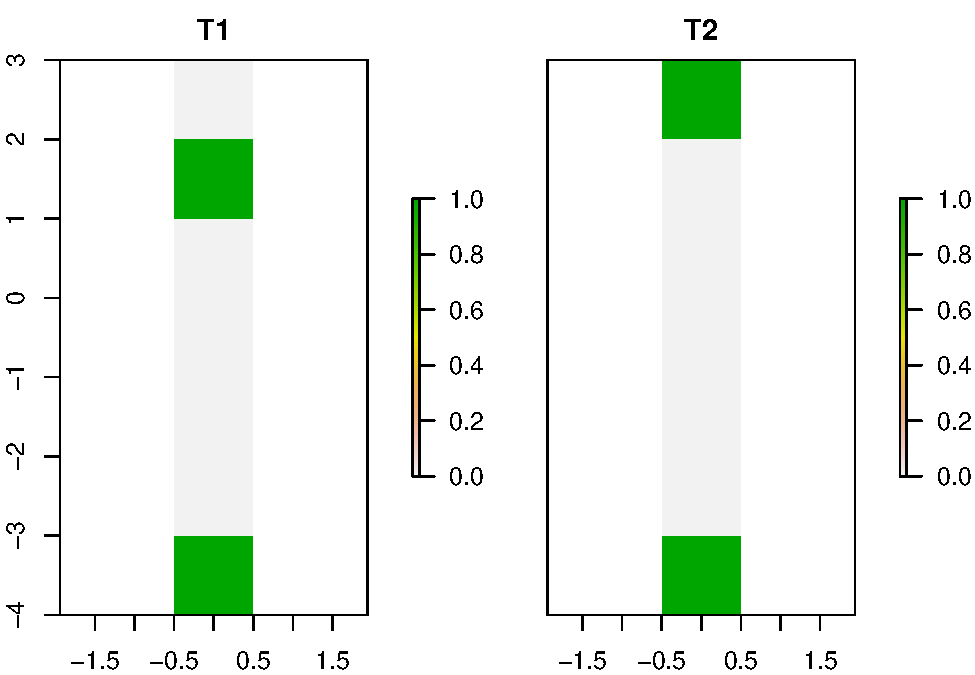
\includegraphics{Ideas2_files/figure-latex/unnamed-chunk-19-1.pdf}
\caption{\label{fig:unnamed-chunk-19}Time slice by time slice solution}
\end{figure}

\begin{figure}
\centering
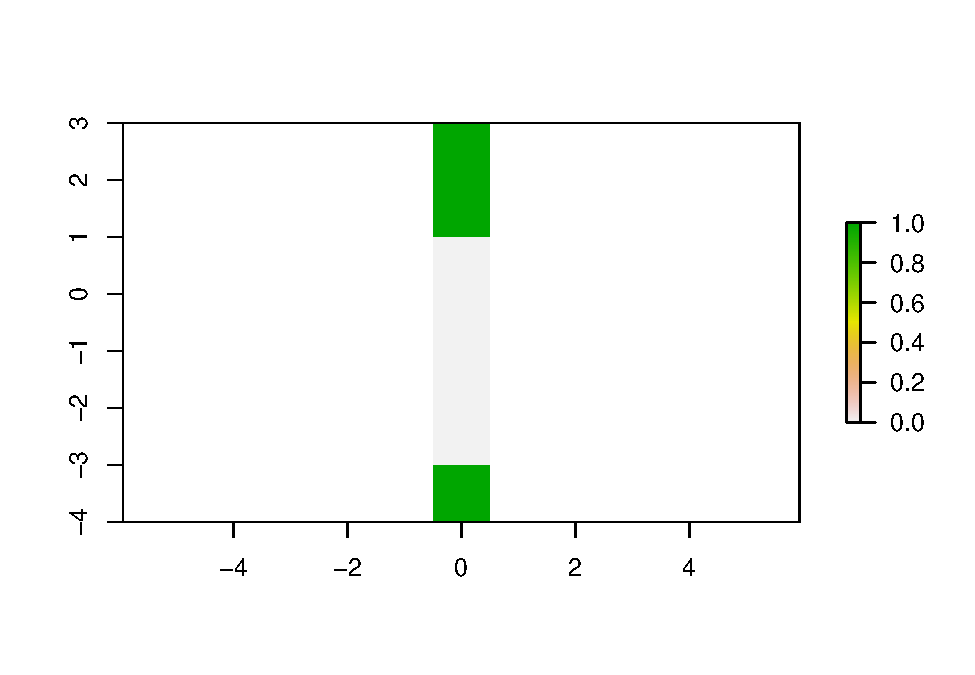
\includegraphics{Ideas2_files/figure-latex/unnamed-chunk-20-1.pdf}
\caption{\label{fig:unnamed-chunk-20}Global solution}
\end{figure}

\hypertarget{quadriatic-solution-for-the-same}{%
\subsection{Quadriatic solution for the same}\label{quadriatic-solution-for-the-same}}

\begin{verbatim}
## 
## Using solver 'cccp' with parameters: 
##          Value
## trace        0
## abstol   1e-06
## feastol  1e-05
## stepadj    0.9
## maxiters   100
## reltol   1e-06
## beta       0.5
\end{verbatim}

\begin{Shaded}
\begin{Highlighting}[]
\NormalTok{edges_solved <-}\StringTok{ }\KeywordTok{bind_cols}\NormalTok{(edges_formatted, }\DataTypeTok{solution =}\NormalTok{ res}\OperatorTok{$}\NormalTok{x) }\OperatorTok\StringTok{ }\KeywordTok{left_join}\NormalTok{(df_IDs) }\OperatorTok\StringTok{ }
\StringTok{    }\NormalTok{dplyr}\OperatorTok{::}\KeywordTok{filter}\NormalTok{(solution }\OperatorTok{!=}\StringTok{ }\DecValTok{0}\NormalTok{) }\OperatorTok\StringTok{ }\KeywordTok{group_by}\NormalTok{(node_to, raster_id, timeslice_to) }\OperatorTok\StringTok{ }
\StringTok{    }\KeywordTok{summarise}\NormalTok{(}\DataTypeTok{solution =} \KeywordTok{sum}\NormalTok{(solution))}


\NormalTok{TestStack <-}\StringTok{ }\KeywordTok{list}\NormalTok{()}


\ControlFlowTok{for}\NormalTok{ (i }\ControlFlowTok{in} \DecValTok{1}\OperatorTok{:}\KeywordTok{nlayers}\NormalTok{(layers_habitat)) \{}
\NormalTok{    Test <-}\StringTok{ }\NormalTok{layer_cost}
    \KeywordTok{values}\NormalTok{(Test) <-}\StringTok{ }\DecValTok{0}
    \KeywordTok{values}\NormalTok{(Test)[edges_solved }\OperatorTok\StringTok{ }\NormalTok{dplyr}\OperatorTok{::}\KeywordTok{filter}\NormalTok{(timeslice_to }\OperatorTok{==}\StringTok{ }\NormalTok{(i)) }\OperatorTok\StringTok{ }\KeywordTok{pull}\NormalTok{(raster_id) }\OperatorTok\StringTok{ }
\StringTok{        }\KeywordTok{unique}\NormalTok{()] <-}\StringTok{ }\NormalTok{edges_solved }\OperatorTok\StringTok{ }\NormalTok{dplyr}\OperatorTok{::}\KeywordTok{filter}\NormalTok{(timeslice_to }\OperatorTok{==}\StringTok{ }\NormalTok{(i)) }\OperatorTok\StringTok{ }\KeywordTok{group_by}\NormalTok{(raster_id) }\OperatorTok\StringTok{ }
\StringTok{        }\KeywordTok{summarise}\NormalTok{(}\DataTypeTok{flow =} \KeywordTok{sum}\NormalTok{(solution)) }\OperatorTok\StringTok{ }\KeywordTok{pull}\NormalTok{(flow)}
\NormalTok{    TestStack[[i]] <-}\StringTok{ }\NormalTok{Test}
\NormalTok{\}}

\NormalTok{TestStack <-}\StringTok{ }\KeywordTok{do.call}\NormalTok{(}\StringTok{"stack"}\NormalTok{, TestStack)}

\KeywordTok{names}\NormalTok{(TestStack) <-}\StringTok{ }\KeywordTok{paste0}\NormalTok{(}\StringTok{"T"}\NormalTok{, }\DecValTok{1}\OperatorTok{:}\KeywordTok{nlayers}\NormalTok{(TestStack))}
\end{Highlighting}
\end{Shaded}

\begin{figure}
\centering
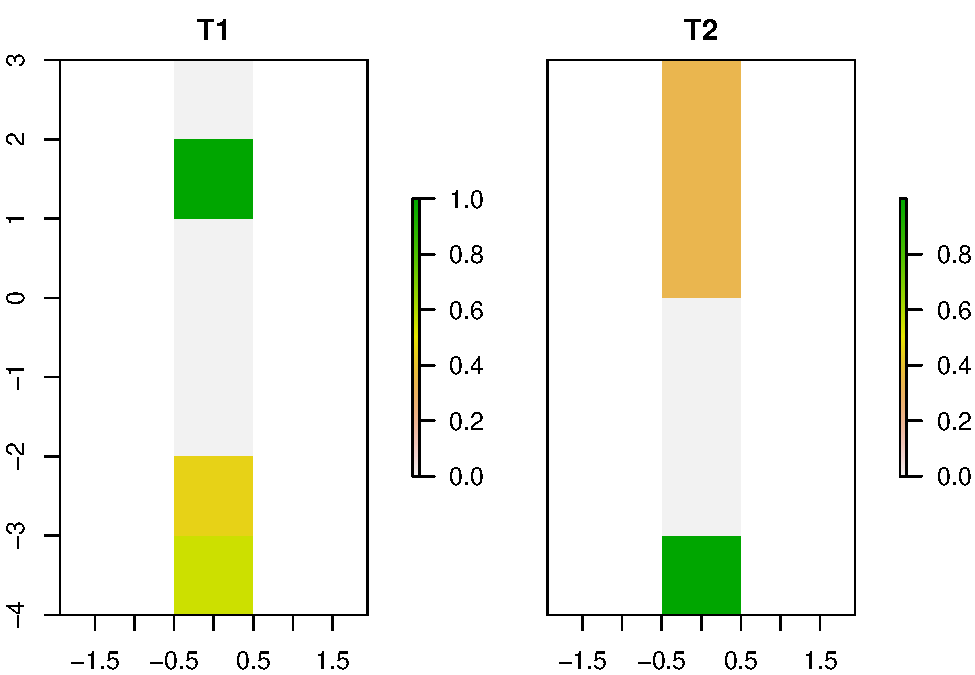
\includegraphics{Ideas2_files/figure-latex/unnamed-chunk-23-1.pdf}
\caption{\label{fig:unnamed-chunk-23}Time slice by time slice quadratic solution}
\end{figure}

\begin{figure}
\centering
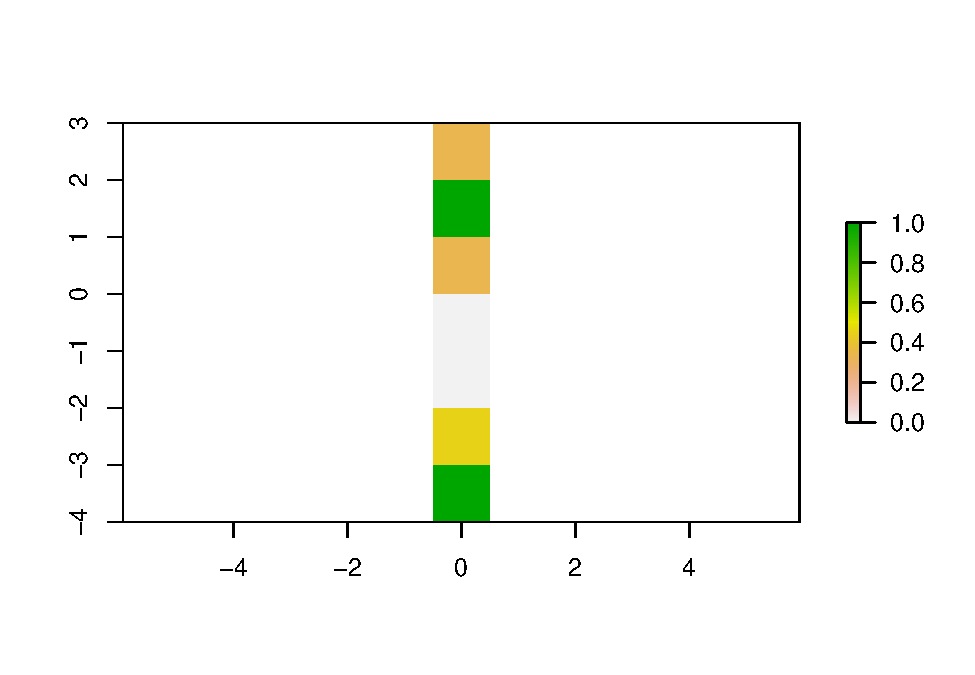
\includegraphics{Ideas2_files/figure-latex/unnamed-chunk-24-1.pdf}
\caption{\label{fig:unnamed-chunk-24}Global quadratic solution}
\end{figure}

\begin{table}[!h]

\caption{\label{tab:SolutionQuad}Solution}
\centering
\begin{tabular}[t]{rrrr}
\toprule
node\_to & raster\_id & timeslice\_to & solution\\
\midrule
\rowcolor{gray!6}  9 & 2 & 1 & 1.0000000\\
13 & 6 & 1 & 0.4545454\\
\rowcolor{gray!6}  14 & 7 & 1 & 0.5454546\\
15 & 1 & 2 & 0.3333333\\
\rowcolor{gray!6}  16 & 2 & 2 & 0.3333333\\
\addlinespace
17 & 3 & 2 & 0.3333333\\
\rowcolor{gray!6}  21 & 7 & 2 & 1.0000000\\
22 & NA & 3 & 2.0000000\\
\bottomrule
\end{tabular}
\end{table}

\end{document}
